\chapter{代理内核实验的参考实现}

在本章节,我们将给出移植K210后的代理内核实验的参考实现。
每个实验实现的阐述结构大致相同,
先从实验预期开始,描述实验的目标和预期效果。
然后我们会给出参考实现的代码和实现过程描述。
最后给出实验执行流程的总结。

\section{系统调用}
你好
\subsection{实验预期}

给定用户态应用user/app\_helloworld.c。
实验的目标是PKE能够加载并成功运行它。
实验预期是应用可以打印出“Hello world!”,并正常退出。

\begin{lstlisting}[caption={用户态应用app\_helloworld.c}, label={lst:app_helloworld}, language=C]
    #include "user_lib.h"

    int main(void) {
        printu("Hello world!\n");
        exit(0);
    }   
\end{lstlisting}

\subsection{具体实现}

如上的用户态代码很简单,只有两行。第一行是用户态的打印函数printu()。
第二行是退出进程的函数exit()。
关于printu()和exit()函数的定义在user\_lib.c。
接下来我们看看这两个函数的具体实现:

\begin{lstlisting}[caption={printu与exit的实现}, label={lst:printu_exit}, language=C]
    int printu(const char *s, ...) {
        va_list vl;
        va_start(vl, s);
        char out[256];  // fixed buffer size.
        int res = vsnprintf(out, sizeof(out), s, vl);
        va_end(vl);
        const char *buf = out;
        size_t n = res < sizeof(out) ? res : sizeof(out);

        return do_user_call(SYS_user_print, (uint64) buf, n, 0, 0, 0, 0, 0);
    }

    int exit(int code) {
        return do_user_call(SYS_user_exit, code, 0, 0, 0, 0, 0, 0);
    }   
\end{lstlisting}

观察发现,printu()和exit()函数的实现都是简单处理了输入的参数,
然后就调用了do\_user\_call()函数。他们俩都是通过系统调用来获取自己所需的功能。
那么结论已经很明显,
我们只需要在PKE的内核代码中实现printu()和exit()的系统调用即可。

观察内核代码发现,printu()和exit()的系统调用都已经实现,
系统调用部分只有handle\_syscall()并未实现。该函数的功能是让用户进程的pc值增加4。
之所以增加4,是因为RISC-V的指令是32位的,32位代表着4个字节。
然后调用系统调用,最终将返回值保存在a0寄存器中。接下来我们给出它的实现代码。

\begin{lstlisting}[caption={handle\_syscall的实现}, label={lst:handle_syscall}, language=C]
static void handle_syscall(trapframe *tf) {
    tf->epc += 4;
    tf->regs.a0 = do_syscall(tf->regs.a0, tf->regs.a1,
                                tf->regs.a2, tf->regs.a3, 
                                tf->regs.a4, tf->regs.a5, 
                                tf->regs.a6, tf->regs.a7);
}
\end{lstlisting}

\begin{figure}[h]
    \vspace{13pt} % 调整图片与上文的垂直距离
    \centering
    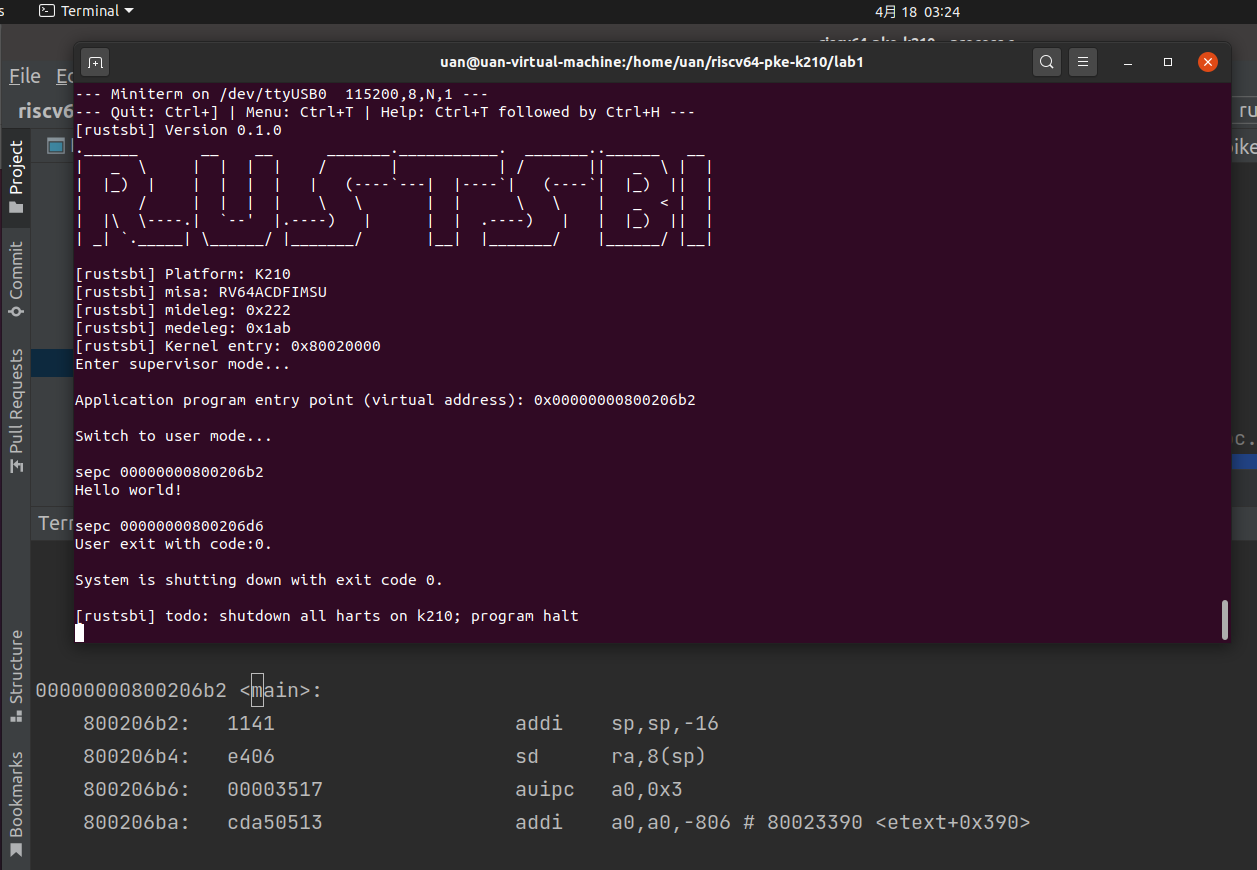
\includegraphics[width=0.9\textwidth]{images/labs/lab1.png}
    \caption{lab1实验结果}\label{lab1实验结果} % label 用来在文中索引
\end{figure}

将实验要求实现后,我们可以在K210上运行实验代码,得到如下结果:

\section{异常处理}

\subsection{实验预期}

\subsection{实验分析}

\section{定时器中断}

\subsection{实验预期}

\subsection{实验改进}

\subsection{具体实现}

\subsection{执行流程}

\section{虚拟地址和物理地址的转换}

\subsection{实验预期}

\subsection{具体实现}

\subsection{执行流程}

\section{基本的内存管理}

\subsection{实验预期}

\subsection{具体实现}

\subsection{执行流程}

\section{栈空间不足与缺页异常}
你好
\subsection{实验预期}

\subsection{具体实现}

\subsection{执行流程}

\section{创建子进程fork的实现}

\subsection{实验预期}

\subsection{兼容K210与改进}

\subsection{具体实现}

\subsection{执行流程}

\section{进程的控制权交接}

\subsection{实验预期}

\subsection{具体实现}

\subsection{执行流程}

\section{进程的时间片调度}

\subsection{实验预期}

\subsection{具体实现}

\subsection{执行流程}

\section{实验资料的编写及管理}

\subsection{实验指导书的编写}

\subsection{实验指导书的管理}

\subsection{对应代码库的管理}
你好
